 
% run the command ' lualatex -shell-escape Reference.tex ' twice in the terminal to visualize table of contents
\documentclass[twoside]{article}
\usepackage[utf8]{inputenc}
\usepackage[spanish]{babel}
\usepackage{geometry}
\usepackage{multicol}
\usepackage{minted}
\usepackage{python}
\usepackage[hidelinks]{hyperref}
\usepackage{fancyhdr}
\usepackage{listings}
\usepackage{pdfpages}
\usepackage{needspace}
\usepackage{sectsty}
\usepackage{array}
\usepackage{multirow} 
\usepackage{longtable}
\usepackage{xcolor}
\usepackage{afterpage}
\usepackage{amssymb}
\usepackage{amsmath}
\usepackage[inline]{enumitem}
\usepackage{graphicx}
\usepackage{float}

\newcommand{\wdir}[1]{/home/san/Algorithms/Reference/#1}
\geometry{letterpaper, portrait, left=0.9cm, right=0.9cm, top=1.8cm, bottom=1.5cm}

\sectionfont{\Huge\bfseries\sffamily}

\definecolor{LightGray}{gray}{0.9}
\definecolor{prussianblue}{rgb}{0.0, 0.19, 0.33}
\definecolor{indigo(dye)}{rgb}{0.0, 0.25, 0.42}
\definecolor{lapislazuli}{rgb}{0.15, 0.38, 0.61}
\definecolor{mediumelectricblue}{rgb}{0.01, 0.31, 0.59}
\definecolor{smalt(darkpowderblue)}{rgb}{0.0, 0.2, 0.6}
\definecolor{yaleblue}{rgb}{0.06, 0.3, 0.57}
\definecolor{skobeloff}{rgb}{0.0, 0.48, 0.45}
\definecolor{pinegreen}{rgb}{0.0, 0.47, 0.44}

\setminted{
    style=tango,
    breaklines=true,
    bgcolor=LightGray
}

\setlength{\headsep}{0.9cm}
\setlength{\columnsep}{0.5cm}
\setlength{\columnseprule}{0.01cm}
\renewcommand{\columnseprulecolor}{\color{gray}}

\pagestyle{fancy}
\pagenumbering{arabic}
\fancyhead{}
\fancyfoot{}
\fancyhead[LO,RE]{\textbf{\textsf{Autor: Sergio Gabriel S\'anchez Valencia}}}
\fancyhead[LE,RO]{\textsf{\leftmark}}
\fancyfoot[LE,RO]{\textbf{\textsf{\thepage}}}
 
\renewcommand{\headrulewidth}{0.01cm}
\renewcommand{\footrulewidth}{0.01cm}

\setlength{\parindent}{0em}
% column space
\setlength{\tabcolsep}{10pt} % Default value: 6pt
% upper and lower padding
\renewcommand{\arraystretch}{1.5} % Default value: 1

\begin{document}
\fontfamily{lmss}
\selectfont
\newpage
\section*{\centering Cuestionario control diseño de bases de datos}
\subsection*{Respuestas}
\begin{enumerate}
      \item Se genera una descomposición con pérdida ya que en las entidades generadas no hay un atributo que
            identifique a la otra entidad de manera única. La propuesta de tal atributo podría ser el nombre, sin embargo
            los nombres se pueden llegar a repetir por lo tanto ese atributo no nos sirve para relacionar ambas entidades generadas.
      \item FALTA
      \item Una superclave es la encargada de identificar a un conjunto de atributos de manera única, mientras
            que una dependencia funcional es un concepto más general para indicar que la existencia de cierto conjunto
            de atributos depende de otro conjunto de atributos.
      \item NO EXISTE
      \item Descomponer una entidad en otras entidades basado en las dependencias funcionales nos permite evitar redundancia
            en los datos y facilitar los procesos de insercion, eliminacion y actualizacion de algun registro en la base de datos.
      \item NO EXISTE
      \item Corregir datos duplicados y anomalías en la base de datos. Evitar la creación y actualización de relaciones y dependencias
            no deseadas entre datos. Prevenir borrados indeseados de datos.Optimizar el espacio de almacenamiento.
            Reducir el tiempo y complejidad de revisión de las bases de datos cuando es necesario introducir nuevos tipos de datos.
            Facilitar el acceso e interpretación de los datos a los usuarios y aplicaciones que los usan.
      \item Puede que existan entidades que por definición se encuentran en la forma Normal de Boyce Codd, sin embargo es notable que
            estas requieren más normalización como es el caso de la entidad inst\_info que se menciona en el libro.
      \item El poder descomponer las entidades a una forma más atómica y el poder identificar las relaciones entre dichas entidades y así
            evitar errores en los diseños de bases de datos.
      \item Es el conjunto de todas las dependencias incluidas en $F$, junto con las dependencias que pueden inferirse de $F$, reciben el nombre
            de clausuras de $F$; está designada mediante $F^+$, donde $F$ es el conjunto de todas las dependencias funcionales de un esquema de relación.
      \item $R = (A, B, C, G, H, I)$ y $F = \{ A \rightarrow B, A \rightarrow C, CG \rightarrow H, CG \rightarrow I, B \rightarrow H \}$
            \begin{enumerate}
                  \item $A \rightarrow H$ (transivity), $AG \rightarrow I$ (augmenting then transitivity), $CG \rightarrow HI$ (augmenting and transitivity)
            \end{enumerate}
      \item Algoritmo para calcular $F^+$
            \begin{enumerate}
                  \item Inicializar $F^+$ con $F$
                  \item Para cada dependencia funcional en $F^+$
                        \begin{enumerate}
                              \item Aplicar reglas de aumentación y reflexividad y añadir las dependencias funcionales resultantes a $F^+$
                        \end{enumerate}
                  \item Para cada par de dependencias funcionales $f_1$ y $f_2$ en $F^+$
                        \begin{enumerate}
                              \item si $f_1$ y $f_2$ pueden ser combinadas usando transitividad entonces añadir la dependencia funcional resultante a $F^+$
                        \end{enumerate}
                  \item repetir desde el paso $b$ hasta que $F^+$ deje de modificarse
            \end{enumerate}
      \item - Reglas de cerradura adicionales:
            \begin{enumerate}
                  \item si $a \rightarrow b$ y $a \rightarrow c$ , entonces $a \rightarrow bc$
                  \item si $a \rightarrow bc$ , entonces $a \rightarrow b$ y $a \rightarrow c$
                  \item si $a \rightarrow b$ y $cb \rightarrow z$ , entonces $ac \rightarrow z$
            \end{enumerate}}
      \item Algoritmo para determinar la cerradura de atributos sobre un conjunto de dependencias funcionales $A$
            \begin{enumerate}
                  \item Inicializar el resultado como $A$.
                  \item repetir mientras haya cambios en el resultado
                        \begin{enumerate}
                              \item para cada dependencia $b \rightarrow c$
                                    \begin{itemize}
                                          \item Si $b$ es un subconjunto del resultado entonces hacer $resultado = resultado \cap c$
                                    \end{itemize}
                        \end{enumerate}
            \end{enumerate}
      \item Verificar la selección de una superclave, verificar las dependencias funcionales y calcular la cerradura de $F$.
      \item NO EXISTE
      \item a cubierta canónica es el mínimo conjunto de dependencias funcionales equivalentes a $F$.
            Sin dependencias redundantes ni partes de dependencias redundantes.

      \item Básicamente si un atributo $A$ se puede eliminar sin afectar la cerradura del conjunto de dependencias funcionales, entonces $A$ es un atributo extraño.
      \item Para probar si un atributo $A$ es extraño en $a \rightarrow b$ en $F$ se hace lo siguiente:
            \begin{enumerate}
                  \item para checar si es extraño en $a$
                        \begin{enumerate}
                              \item calcular $(\{a\} - A)^+$ usando dependencias de $F$
                              \item si $(\{a\} - A)^+$ contiene a $b$, entonces $A$ es extraño en $a$
                        \end{enumerate}
                  \item para checar si es extraño en $b$
                        \begin{enumerate}
                              \item calcular $a^+$ usando solo dependencias de en $F' = (F - \{a \rightarrow b\}) \cup \{a \rightarrow (b - A)\}$
                              \item si $a^+$ contiene a $A$, entonces $A$ es extraño en $b$
                        \end{enumerate}
            \end{enumerate}
      \item La cubierta canonica para $F$ es un conjunto de dependencias $F_c$ tal que:
            \begin{enumerate}
                  \item $F$ implica logicamente todas las dependencias de $F_c$
                  \item $F_c$ implica todas las dependencias de $F$
                  \item Ninguna dependencia en $F_c$ contiene un atributo extraño
                  \item El lado izquierdo de todas las dependencias funcionales en $F_c$ es único.
            \end{enumerate}
      \item La descomposición sin pérdidas implica que al dividir una relación en 2 o más relaciones, se puede regresar a la relación
            original con la unión natural de las relaciones generadas.
      \item Para checar si una dependencia $a \rightarrow b$ se preserva en una descomposición de $R$ en $R1, R2, \cdots, Rn$ aplicamos las siguientes pruebas:
            \begin{enumerate}
                  \item inicializamos el resultado en $a$
                  \item repetir mientras haya cambios en el resultado:
                        \begin{enumerate}
                              \item Para cada $R_i$ en la descomposición
                                    \begin{enumerate}
                                          \item $t$ = $(resultado \cap R)^+ \cap R_i$
                                          \item $resultado = resultado \cup t$
                                    \end{enumerate}
                        \end{enumerate}
                  \item si el resultado contiene todos los atributos en $b$, entonces la dependencia funcional $a \rightarrow b$ se preserva.

            \end{enumerate}
      \item Para checar si una dependencia no trivial $a \rightarrow b$ causa una violación a la BCNF
            \begin{enumerate}
                  \item caluclar $a^+$
                  \item verificar que incluya todos los atributos de $R$, es decir, que sea una superclave en $R$.
            \end{enumerate}
      \item Algoritmo BCNF
            \begin{enumerate}
                  \item Inicializar $resultado$ con $R$
                  \item Iniciliazar una variable $DONE = falso$
                  \item repetir mientras $DONE$ sea $falso$
                        \begin{enumerate}
                              \item Si existe un esquema $R_i$ en $resultado$ que no esta en BCNF, entonces para cada dependencia $a \rightarrow b$ en $R_i$, tal que $a \rightarrow R_i$ no este en $R^+$ hacer:
                                    \begin{enumerate}
                                          \item $resultado = (resultado - R) \cup (R_i - b) \cup (a, b)$
                                    \end{enumerate}
                              \item sino existe hacer $DONE = verdadero$
                        \end{enumerate}
            \end{enumerate}
      \item $R = (A, B, C), F = \{ A \rightarrow B, B \rightarrow C \} key = \{A\}$
            \begin{enumerate}
                  \item $R$ no esta en BCNF ($B \rightarrow C$, $B$ no es una superclave)
                  \item descomponemos en $R_1$ y $R_2$
                        \begin{enumerate}
                              \item $R_1 = (B, C)$
                              \item $R_2 = (A, B)$
                        \end{enumerate}
            \end{enumerate}
      \item Ejemplo de descomposición en 3NF
            \begin{enumerate}
                  \item Esquema:
                        \begin{enumerate}
                              \item cust\_banker\_branch = (customer\_id, employee\_id, branch\_name, type)
                        \end{enumerate}
                  \item Dependencias Funcionales:
                        \begin{enumerate}
                              \item customer\_id, employee\_id  \rightarrow  branch\_name, type
                              \item employee\_id \rightarrow branch\_name
                              \item customer\_id, branch\_name $\rightarrow$ employee\_id
                        \end{enumerate}
                  \item primero calculamos la cubierta canónica
                        \begin{enumerate}
                              \item branch\_name es extraño en el lado derecho de la primer dependencia, porque podemos determinar branch\_name con solo employee\_id
                              \item Obtenemos Fc =
                                    \begin{enumerate}
                                          \item customer\_id, employee\_id \rightarrow type
                                          \item employee\_id \rightarrow branch\_name
                                          \item customer\_id, branch\_name \rightarrow employee\_id
                                    \end{enumerate}
                        \end{enumerate}
                  \item El bucle genera el siguiente esquema 3NF:
                        \begin{enumerate}
                              \item (Customer\_id, employee\_id, type)
                              \item (\underline{employee\_id}, branch\_name)
                              \item (customer\_id, branch\_name, employee\_id)
                        \end{enumerate}
                  \item El esquema simplificado resultante es:
                        \begin{enumerate}
                              \item (customer\_id, employee\_id, type)
                              \item (customer\_id, branch\_name, employee\_id)
                        \end{enumerate}
            \end{enumerate}
      \item El propósito de una base de datos relacional es:
            \begin{enumerate}
                  \item BCNF
                  \item Descomposición sin pérdidas
                  \item Preservación de las dependencias
            \end{enumerate}
      \item Las dependencias multivaluadas se generan cuando un atributo $A$ determina a otro, pero este no siempre tiene los mismos valores debido a $A$. Un ejemplo seria:
            \begin{figure}[htb]
                  \begin{center}
                        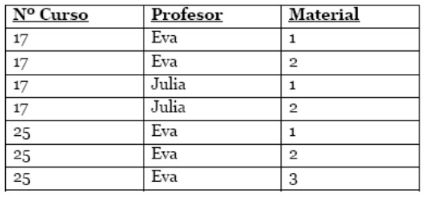
\includegraphics[scale=0.6]{multivalue.png}
                        \caption{Ejemplo de dependencias multivaluadas}
                  \end{center}
            \end{figure}
      \item Formas en las que se utilizan dependencias multivaluadas:
            \begin{enumerate}
                  \item Para determinar si las relaciones son legales bajo un conjunto de dependencias funcionales y dependencias multivalor.
                  \item Para especificar reglas en un conjunto de relaciones legales.
            \end{enumerate}
      \item Características de las teorías de dependencias
            \begin{enumerate}
                  \item Podemos calcular $D^+$ usando $D$, usando definiciones formales de dependencias funcionales y multivalor
                  \item Podemos arreglarnoslas para dependencias muy simples.
                  \item Para dependencias más complejas es mejor razonar usando un sistema de inferencia de reglas.
            \end{enumerate}
      \item Un esquema de relaciones $R$ está en 4NF con respecto al conjunto $D$, de dependencias funcionales y multivalor si para todas las dependencias
            multivalor en $D^+$ de la forma $a \rightarrow \rightarrow b$ donde $a$ y $b \subseteq R$, al menos una de las siguientes condiciones se cumple:
            \begin{enumerate}
                  \item $a \rightarrow \rightarrow b$ es trivial(i.e. $b \subseteq R$ ó $a \cup b = R$)
                  \item $a$ es una superclave en el esquema $R$
                  \item si una relación está en 4NF está en BCNF
            \end{enumerate}
      \item $R = (A, B, C, G ,H, I)$ $F = \{  A \rightarrow  \rightarrow B, B \rightarrow  \rightarrow HI, CG \rightarrow  \rightarrow H  \}$
            \begin{enumerate}
                  \item $R1 =  (A, B)$
                  \item $R2 = (A, C, G, H, I)$
                  \item $R3 = (C, G, H)$
                  \item $R4 = (A, C, G, I)$
                  \item $R5 = (A, I)$
                  \item $R6 = (A, C, G)$
            \end{enumerate}
      \item Mayor velocidad de acceso
\end{enumerate}

\subsection*{Ejercicios}
\subsubsection*{8.11}
\begin{enumerate}
      \item \alpha tiene que ser una clave primaria para $R_1$ y \alpha tiene que ser una clave
            foranea desde $R_2$ referenciando a $R_1$.
      \item Si la restricci\'on de la clave foranea no se aplica, entonces al hacer la eliminación
            de algún registro esta eliminacion no se propagaria adecuadamente por lo que puede significar
            que esta siga existiendo en la BD de alguna manera no deseada.
      \item Para cada esquema $r_i$ (\alpha \beta) añadido al esquema principal por alguna regla $\alpha \rightarrow \beta$, $\alpha$
            deberia convertirse en una llave primaria.\\
            Las llaves foraneas se crean asi: para cada relacion $r_i$ creada por lo anterior, si los atributos the la llave primaria en
            $r_i$ tambien ocurren en otra relacion $r_j$, entonces la llave foranea se crea a partir de esos atributos en $r_j$, haciendo
            referencia a la llave primaria en $r_i$.
\end{enumerate}
\subsubsection*{8.12}
Si $U = R_1, R_2, \cdots R_n$ es un esquema de descomposici\'on y $u(U)$ es una relaci\'on y adem\'as
$r_i = \Pi_{R_I}(u)$. Demostrar que:

$$u \subseteq r_1 \bowtie r_2 \bowtie \cdots \bowtie r_n$$

Consideremos alguna tupla $t$ en $u$.\\
Notemos que $r_i = \Pi_{R_i}(u)$ implica que $t[R_i] \in r_i, 1 \leq i \leq n$. Por lo tanto,\\
$$t[R_1] \bowtie t[R_2] \bowtie \cdots \bowtie t[R_n] \in r_1 \bowtie r_2 \bowtie r_3 \cdots \bowtie \r_n$$
Por definici\'on de la unión natural tenemos que\\
$$t[R_1] \bowtie t[R_2] \bowtie \cdots \bowtie t[R_n] = \Pi_{\alpha} (\sigma_{\beta}(t[R_1] \times t[R_2] \times \cdots \times t[R_n]))$$
Donde la condici\'on \beta se satisface si los valores de los atributos con el mismo nombre en una tupla son iguales y $\alpha = U$.
El producto cartesiano de tuplas individuales genera un tupla. La selección dle proceso se satisface por que todos los atributos
con el mismo nombre tiene que tener el mismo valor ya que son proyecciones de la misma tupla. Finalmente la proyecci\'on elimina
nombres de atributos duplicados.\\

Por la definici\'on de la descomposici\'on, $U = R_1 \cup R_2 \cup \cdots \cup R_n$, lo que significa que todos los atributos de $t$
estan en $t[R_1] \bowtie r[R_2] \bowtie \cdots \bowtie t[R_n]$. Lo que a su vez significa que $t$ es igual al resultado de esta uni\'on.
Ya que $t$ es cualquier tupla arbitraria en $u$,

$$u \subseteq r_1 \bowtie r_2 \bowtie \cdots \bowtie r_n$$

\subsubsection*{8.19}
Del ejercicio 8.6, sabemos que $B \rightarrow D$ no es trivial ya que el lado izquierdo no es una superllave.
Por el algoritmo de la descomposici\'on en BCNF. Deducimos las relaciones $\{(A, B, C, E,), (B, D)\}$. Y estas se encuentran
en BCNF.
\subsubsection*{8.20}
Primero notamos que las dependencias dadas en el ejercicio practica 8.1 forman una cubierta canonica. Por lo que
al aplicar el algoritmo de descomposici\'on sin perdidas a 3NF ya no es necesario generar la cubierta canonica y
por lo tanto siguiendo ese mismo algoritmo nos queda:
$$R' = \{(A, B, C), (C, D, E), (B, D), (E, A)\}$$.
\subsubsection*{8.21}
Normalice el siguiente esquema con las relgas indicadas a 4NF
\begin{itemize}
      \item $books(accessionno, isbn, title, author, publisher)$
      \item $users(userid, name, deptid, deptname)$
      \item $accessionno \rightarrow isbn$
      \item $isb \rightarrow title$
      \item $isbn \rightarrow publisher$
      \item $isbn \rightarrow \rightarrow author$
      \item $userid \rightarrow name$
      \item $userid \rightarrow deptid$
      \item $deptid \rightarrow deptname$
\end{itemize}

\textbf{Respuesta:}\\

En $books$, vemos que:
$$isbn \rightarrow \rightarrow title, publisher, author$$

sin embargo $isbn$ no puede ser una llave primaria, ya que debido a las dependencias multivalor,
$isbn$ apareceria repetidas veces por lo que debemos dividir esta relaci\'on en ($books$) en
otras 2 relaciones:

$$books\_accnno(accessionno, isbn)$$
$$books\_details(isbn, title, publisher, author)$$

despues de esto tenemos todavia que $isbn \rightarrow \rightarrow author$ y dado que como un solo $isbn$
puede tener varios $author$ entonces $isbn$ apareceria repetidas veces en la relaci\'on $book\_details$,
por lo que $isbn$ no puede ser una llave primaria y ninguno de los otros atributos lo son, entonces tenemos
que dividir esta relaci\'on aun mas.

$$books\_details1(isbn, title, publisher)$$
$$books\_authors(isbn, author)$$

Por otro lado en la relaci\'on usuarios vemos que:

$$deptid \rightarrow deptname$$

y $deptid$ no es una superllave por lo que tendremos que extender esa dependencia funcional a otra relaci\'on

$$users(userid, name, deptid)$$
$$deparments(deptid, deptname)$$

y ya no quedan mas dependencias funcionales que se puedan derivar ni tampoco dependencias multivalor que causen
la violación de la 4NF por lo que el conjunto final de relaciones queda asi:

$$books\_accnno(accessionno, isbn)$$
$$books\_details1(isbn, title, publisher)$$
$$books\_authors(isbn, author)$$
$$users(userid, name, deptid)$$
$$deparments(deptid, deptname)$$


\subsubsection*{8.22}
La repetici\'on de los datos en una BD genera mas uso del espacio en memoria, hace dificil mantener consitencia en la BD.
ya que hay que hacer actualizaciones en varias relaciones.
\subsubsection*{8.23}
Algunas dependencias funcionales son llamadas triviales por que estas dependencias funcionales se cumplen para todas las relaciones.

\subsubsection*{8.24}

\subsubsection*{8.25}

Ejemplo contradictorio:
$$persona(nss, curp, nombre)$$

Podemos observar que $nss$ (numero de seguridad social) determina el $nombre$ de una persona, y podemos observar
tambien que el curp determina el $nombre$ de esa misma persona, sin embargo el $nss$ NO determina el $curp$ ni el
$curp$ determina el $nss$

\subsubsection*{8.26}
Demostrar por leyes de Armstrong la regla de la descomposici\'on que indica que:\\
Si $\alpha \rightarrow \beta \gamma$, entonces $\alpha \rightarrow \beta$ y $\alpha \rightarrow \gamma$\\

$\alpha \rightarrow \beta \gamma$\\
$\beta \gamma \rightarrow \beta$ regla de reflexividad\\
$\alpha \rightarrow \beta$ regla de transitividad\\
$\beta \gamma \rightarrow \gamma$ regla de reflexividad\\
$\alpha \rightarrow \gamma$ regla de transitividad\\
\subsubsection*{8.27}
Computar $B^+$ del ejercicio de practica 8.6:\\
Comenzamos con $resultado = \{B\}$. Considerando las DFs de la forma $\beta \rightarrow \gamma$, encontramos que
las unicas dependencias que satisfacen que $\beta \subseteq resultado$ son $B \rightarrow B$ y $B \rightarrow D$
Por lo tanto $B^+ = resultado = \{B, D\}$.
\subsubsection*{8.28}
Demostrar por contradicci\'on que la descomposici\'on del ejercicio practica 8.1 tiene perdida en la uni\'on.\\
\newline
Definamos $r$ como:
\begin{figure}[H]
      \begin{center}
            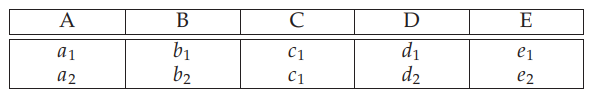
\includegraphics[scale=0.6]{tabla1.png}
      \end{center}
\end{figure}
Con $R_1 = (A, B, C)$ y $R_2 = (C, D, E)$\\
\begin{enumerate}
      \item $\Pi_{R_1}(r)$ seria:
            \begin{figure}[H]
                  \begin{center}
                        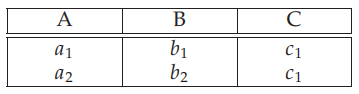
\includegraphics[scale=0.6]{tabla2.png}
                  \end{center}
            \end{figure}
      \item $\Pi_{R_2}(r)$ seria:
            \begin{figure}[H]
                  \begin{center}
                        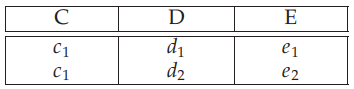
\includegraphics[scale=0.6]{tabla3.png}
                  \end{center}
            \end{figure}
      \item $\Pi_{R_1}(r) \bowtie \Pi_{R_2}(r)$ seria:

            \begin{figure}[H]
                  \begin{center}
                        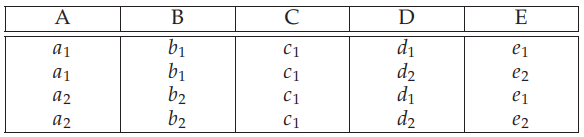
\includegraphics[scale=0.6]{tabla4.png}
                  \end{center}
            \end{figure}
\end{enumerate}
Lo que hace evidente que $\Pi_{R_1}(r) \bowtie \Pi_{R_2}(r) \neq r$, por lo que es una descomposici\'on con perdida

\subsubsection*{8.29}

\subsubsection*{8.30}
Listar 3 objetivos en el diseño de base de datos relacionales.\\
\begin{enumerate}
      \item Descomposición sin perdidas
      \item Preservación de las dependencias
      \item Minimizaci\'on de la repetici\'on de los datos.
\end{enumerate}

\includepdf[pages={1-}]{preguntas.pdf}
\end{document}
